% -----------------------------------------------------------------------------
% Project: PhD KAPPA
% File: kappa.Rnw (root file)
% Author: Alessio Crippa
% Template: based on the tex code written by Andrea Discacciati
%           url: https://github.com/anddis/phd-thesis
%
% Purpose: Root Rnw file, compile this to typeset the kappa!
% -----------------------------------------------------------------------------



% If you get the following error:
%  Error in ensurePackageSymlink(source, target) :
% run the next line, an then restart your R session
% unlink("packrat/lib-R", recursive = TRUE)


% Class
\documentclass[11pt,a4paper,twoside,openany]{book}\usepackage{knitr}

% Packages
\usepackage[english]{babel}
\usepackage{amsfonts}
\usepackage{amsmath}
\usepackage{mathtools}
\usepackage{threeparttable}
\usepackage{adjustbox}
\usepackage{natbib}
\usepackage{graphicx}
\usepackage{flafter}
\usepackage{fancyhdr}
\usepackage{textcomp}
\usepackage[utf8]{inputenc}
\usepackage{setspace}
\usepackage[pdftex,
            pdfauthor={Alessio Crippa},
            pdftitle={Novel methods for dose--response meta-analysis},
            pdfcreator={LaTeX2e}]{hyperref}
\usepackage[%showframe,
			headheight=13.6pt,
			%headsep=,
			%footskip=,
			bindingoffset=0cm,%print=.5cm, web=0cm
			left=3cm,  %print=2cm, web=3cm
			bottom=3cm, %print=3cm, web=3cm
			top=3cm, %print=3cm, web=3cm,
			right=3cm]{geometry} %print=3.5cm, web=3cm
\usepackage{enumerate, mdwlist}
\usepackage{etoolbox}
\usepackage{tabularx}
\usepackage{rotating}
\usepackage[font={small}]{caption}
\usepackage{chngcntr}
\counterwithout{footnote}{chapter}

%---begin see http://www.khirevich.com/latex/font/
\usepackage[activate={true,nocompatibility},final,tracking=true,kerning=true,spacing=true,factor=1100, stretch=10,shrink=10]{microtype}
% remove warning
\microtypecontext{spacing = nonfrench}
\usepackage[T1]{fontenc}
% remove warning
\global\expandafter\let\csname ver@amsfonts.sty\endcsname\relax
% remove issue related to interwordspace
\setlength{\emergencystretch}{10pt}
\usepackage[bitstream-charter]{mathdesign}
\usepackage{sectsty}
	\chapterfont{\usefont{T1}{qhv}{b}{n}\selectfont\huge}
\usepackage{titlesec}

% ---------------------------------------------------------
% Project: PhD KAPPA
% File: _titlesec.tex
% Author: Andrea Discacciati
%
% Purpose: Headings format
%			(see titlesec package)
% ---------------------------------------------------------

\titleformat{\section}[hang]{
    \usefont{OT1}{qhv}{bx}{n}\selectfont}
    {} 
    {0em}
    {\hspace{-0.4pt}\Large \thesection\hspace{0.6em}}
\titleformat{\subsection}[hang]{
    \usefont{OT1}{qhv}{bx}{n}\selectfont}
    {} 
    {0em}
    {\hspace{-4pt} \thesubsection\hspace{0.6em}}
\titleformat{\subsubsection}[hang]{
    \usefont{OT1}{qhv}{bx}{n}\selectfont}
    {} 
    {0em}
    {\normalsize}
\usepackage{tocloft}

% ---------------------------------------------------------
% Project: PhD KAPPA
% File: _tocloft.tex
% Author: Andrea Discacciati
%
% Purpose: Table of Contents, 
%			List of Figures, List of Tables format
%			(see tocloft package)
% ---------------------------------------------------------

\renewcommand{\cfttoctitlefont} % ToC title
             {\usefont{T1}{qhv}{b}{n}\selectfont\huge}
\renewcommand{\cftchapfont} % chapter titles
             {\usefont{T1}{qhv}{b}{n}\selectfont}
\renewcommand{\cftsecfont} % section titles
             {\usefont{T1}{bch}{m}{n}\selectfont}
\renewcommand{\cftsubsecfont} % subsection titles
             {\usefont{T1}{bch}{m}{n}\selectfont} 
\renewcommand{\cftchappagefont} % chapter page numbers
             {\usefont{T1}{bch}{b}{n}\selectfont}
\renewcommand{\cftsecpagefont} % section page numbers
             {\cftsecfont} 
\renewcommand{\cftsubsecpagefont} % subsection page numbers
             {\cftsubsecfont}
             
\renewcommand{\cftloftitlefont} % LoF title
             {\usefont{T1}{qhv}{b}{n}\selectfont\huge}
\renewcommand{\cftfigfont} % Figures titles
             {\usefont{T1}{bch}{m}{n}\selectfont}
             
\renewcommand{\cftlottitlefont} % LoT title
             {\usefont{T1}{qhv}{b}{n}\selectfont\huge}
\renewcommand{\cfttabfont} % Tables titles
             {\usefont{T1}{bch}{m}{n}\selectfont}
%---end see http://www.khirevich.com/latex/font/

% Header / footer

% ---------------------------------------------------------
% Project: PhD KAPPA
% File: _fancyhdr.tex
% Author: Alessio Crippa
% based on the template written by Andrea Discacciati
%
% Purpose: Header and footer settings
%			(see fancyhdr package)
% ---------------------------------------------------------

\pagestyle{fancy}
\renewcommand{\chaptermark}[1]{%
 \markboth{{\thechapter.\ #1}}{}}

\fancypagestyle{plain}{%
  \fancyhf{}%
  \renewcommand{\headrulewidth}{0pt}%
  \fancyhf[lef,rof]{}%
  %\fancyhead[LE,RO]{\thepage}
}

\fancypagestyle{frontmatter}{%
  \renewcommand{\headrulewidth}{0pt} 
  \renewcommand{\footrulewidth}{0pt}
  \fancyhf{}% Clear header/footer
  \fancyhead[LE,RO]{}
}

\fancypagestyle{nothing}{%
  \renewcommand{\headrulewidth}{0pt} 
  \renewcommand{\footrulewidth}{0pt}
  \fancyhf{}% Clear header/footer
  \fancyhead[LE,RO]{}%
}

\fancypagestyle{mainmatter}{%
  \renewcommand{\headrulewidth}{.4pt}
  \renewcommand{\footrulewidth}{0pt}
  \fancyhf{}% Clear header/footer
  \fancyhead[LE,RO]{\thepage}
  \fancyhead[RE,LO]{\nouppercase \leftmark}
}

	
% See 'writing a thesis with latex' p25 
% Writes nothing on empty pages
\makeatletter
\def\cleardoublepage{\clearpage\if@twoside
\ifodd\c@page
\else\hbox{}\thispagestyle{empty}\newpage
\if@twocolumn\hbox{}\newpage\fi\fi\fi}
\makeatother

% Substitutions (%examples)
%\newcommand{\rveplot}{decorrelated-residuals--versus--exposure plot}
%\newcommand{\kgmsq}{kg$\times$m\textsuperscript{$-2$}}

\defcitealias{crippadosresmeta2016}{Paper~I}	
\defcitealias{discacciati2015goodness}{Paper~II}	
\defcitealias{crippa2016new}{Paper~III}	
\defcitealias{crippa2018pointwise}{Paper~IV}	
\defcitealias{crippa2018one}{Paper~V}	

%\doublespacing 
\onehalfspacing

\allowdisplaybreaks

\renewcommand{\sfdefault}{qhv}
\newcommand*{\LargerCdot}{\raisebox{-0.25ex}{\scalebox{1.2}{$\cdot$}}}

\DeclareMathOperator{\R}{\textsf{R}}
\DeclareMathOperator{\Cov}{Cov} 
\DeclareMathOperator{\diag}{diag} 
\DeclareMathOperator{\N}{N} 
\DeclareMathOperator{\E}{E}
\DeclareMathOperator{\logit}{logit} 
\DeclareMathOperator{\df}{df} 
\hyphenation{logRRs}
\hyphenation{logRR}

\addto\captionsenglish{%
  \renewcommand{\bibname}{References}%
}

%\includeonly{abstract, results, introduction, background, aims, discussion, conclusions }

%--- Kappa starts here! ---%
\IfFileExists{upquote.sty}{\usepackage{upquote}}{}
\begin{document}

% Front matter
\frontmatter
\pagestyle{nothing}

% ---------------------------------------------------------
% Project: PhD KAPPA
% File: titlepage.tex
% Author: Alessio Crippa
% based on the template written by Andrea Discacciati
%
% Purpose: Custom title page + ISBN/copyright page
% ---------------------------------------------------------

\begin{titlepage}
\newgeometry{margin=4cm}
\begin{center}
\large
From the Department of Public Health Sciences \\
Karolinska Institutet, Stockholm, Sweden        
\vfill
\Large
\textbf{\textsf{NOVEL METHODS FOR DOSE-RESPONSE META-ANALYSIS}}
\vfill
\Large
Alessio Crippa
\vfill

\includegraphics[width=0.8\textwidth]{figures/ki-logo_pos}
\vfill
\large
Stockholm 2018        
\end{center}
\restoregeometry
\end{titlepage}

\newpage
\null
\vfill
\noindent All published papers reproduced with permission \\
%Cover illustration ``Portraits of sophistication'' by Lamai McCartan \\
Published by Karolinska Institutet \\
\bigskip
Printed by E-Print AB 2018 \\
Edited in R using knitr \\
\textcopyright Alessio Crippa, 2018 \\
ISBN <include number>
\newpage

% ---------------------------------------------------------
% Project: PhD KAPPA
% File: spikblad.tex
% Author: Alessio Crippa
% based on the template written by Andrea Discacciati
%
% Purpose: Spikblad
% ---------------------------------------------------------
\null
\vspace{1.5cm}
\noindent{\Large \textsf{NOVEL METHODS FOR DOSE-RESPONSE META-ANALYSIS} \vspace{1cm}}\\
\noindent{\Large \textsf{THESIS FOR DOCTORAL DEGREE (Ph.D.)} \vspace{.5cm}}\\
By \vspace{.5cm} \\
{\Large \textbf{\textsf{Alessio Crippa}} \vspace{2cm}}\\
\begin{minipage}[t]{6.2cm}
\singlespacing
{\small
\textit{Principal supervisor:}\\
Associate Professor Nicola Orsini \\
Karolinska Institutet \\
\bigskip
Department of Public Health Sciences \\
\textit{Co-supervisor:}\\
Professor Alicja Wolk \\
Karolinska Institutet \\
\medskip
Institute of Environmental Medicine \\
Professor Matteo Bottai \\
Karolinska Institutet \\
\medskip
Institute of Environmental Medicine \\
Professor Donna Spiegelman \\
Harvard T.H. Chan School of Public Health \\
Department of Epidemiology
}
\end{minipage}
\hspace{1.5cm}
\begin{minipage}[t]{8.1cm}
\singlespacing
{\small
\textit{Opponent:}\\
Professor Christopher H. Schmid \\
Brown University \\
Center for Evidence Based Medicine\bigskip \\
\textit{Examination board:}\\
Associate Professor Nele Brusselaers \\
Karolinska Institutet \\
Department of Microbiology, Tumor and Cell Biology \medskip \\
Associate Professor Antonio Gasparrini \\
London School of Hygiene and Tropical Medicine \\
Department of Social $\&$ Environmental Health Research\medskip \\
Professor Paul Lambert \\
University of Leicester \\
Department of Health Sciences
}
\end{minipage}
\cleardoublepage

% ---------------------------------------------------------
% Project: PhD KAPPA
% File: dedication.tex
% Author: Alessio Crippa
% based on the template written by Andrea Discacciati
%
% Purpose: Dedication
% ---------------------------------------------------------

\begin{flushright}
%http://pubmedcentralcanada.ca/pmcc/articles/PMC2550765/pdf/bmj00610-0065.pdf
\null\vspace{\stretch{1}}
\textit{``The function of the expert reviewer is not to be more right than other people, \\
but to be wrong for more sophisticated reasons.''} \\
---Iain Chalmers and Douglas G. Altman \\ 
\textit{Systematic Reviews}, 1995
\vspace{\stretch{2}}\null
\end{flushright}


\iffalse
\begin{flushright}
\null\vspace{\stretch{1}}
\textit{``If I have seen further, it is by standing on the shoulders of giants.''} \\
---Isaac Newton
\vspace{\stretch{2}}\null
\end{flushright}
\fi
\cleardoublepage 
\pagestyle{frontmatter}

% ---------------------------------------------------------
% Project: PhD KAPPA
% File: abstract.tex
% Author: Andrea Discacciati
%
% Purpose: Abstract frontmatter
% ---------------------------------------------------------


\noindent {\Large \textsf{\textbf{{Abstract}}}
\bigskip
%\chapter*{Abstract}
\small
\par Dose-response meta-analysis is a statistical technique increasingly used to combine and contrast the evidence on the association between a continuous exposure and the risk of a health outcome. Several papers refined selected aspects of the methodology, such as implementations of flexible strategies and considering extensions to multivariate meta-analysis. However, there were still several relevant questions that needed to be addressed. This thesis aims to address these issues by developing and implementing (\citetalias{crippadosresmeta2016}) new strategies and ad-hoc measures, including tools for evaluating the goodness-of-fit (\citetalias{discacciati2015goodness}), a new measure for quantifying the impact of heterogeneity (\citetalias{crippa2016new}), a strategy to deal with differences in the exposure range across studies (\citetalias{crippa2018pointwise}), and a one-stage approach to estimate complex models without excluding relevant studies (\citetalias{crippa2018one}).

In \citetalias{crippadosresmeta2016}, we described the implementation of the main aspects of the methodology in the \texttt{dosresmeta} $\R$ package available on CRAN. Dedicated functions was written to facilitate specific tasks such as definition of the design matrix and prediction of the pooled results. We illustrated how to estimate both linear and non-linear curves, conduct test of hypotheses, and present the results in a grapichal way using summarized data on alcohol intake and colorectal cancer risk.
 
In \citetalias{discacciati2015goodness}, we discussed how to evaluate the goodness-of-fit for dose-response meta-analysis. The proposed solutions consist of descriptive measures to summarize the agreement between fitted and observed data (the deviance and the coefficient of determination), and graphical tools to visualize the fit of the model (decorrelated residuals-versus-exposure plot). Data from two published meta-analyses were used to show how these tools can improve the practice of quantitative synthesis of aggregated dose-response data. 

In \citetalias{crippa2016new}, we proposed and discussed a new measure, $R_b$, to quantify the proportion of the variance of the pooled estimate attributable to the between-study heterogeneity. $R_b$ does not make any assumption about the distribution of the within-study error variances, nor does it require specification of a typical value for these quantities. The performance of the proposed measure was evaluated in an extensive simulation study. We demonstrated how to present and interpret the $R_b$ re-analyzing three published meta-analyses.

In \citetalias{crippa2018pointwise}, we extended a point-wise approach to dose--response meta-analysis of aggregated data. The strategy consists of combining predicted relative risks for a fine grid of exposure values based on potentially different dose-response models. Thus, a point-wise approach can improve the flexibility in modelling the study-specific curves and may limit the impact of extrapolation by predicting the study-specific relative risk based on the observe exposure range. We illustrated the methodology using both individual and aggregated participant data.

In \citetalias{crippa2018one}, we formalized a one-stage approach for dose--response meta-analysis in terms of a linear mixed model. We explained the main aspects of the methodology and how to extend the measures typically presented in a two-stage analysis. Using both hypothetical and real data, we showed how the one-stage approach can facilitate investigation the impact of heterogeneity over the exposure range, model comparison, and prediction of individual dose-response associations. The main advantage is that complex curves can be estimated without excluding relevant studies.

In conclusion, the methods presented in this thesis enrich the set of tools available to apply dose--response meta-analyses and to address specific questions including goodness-of-fit evaluation (\citetalias{discacciati2015goodness}) and a new measure of heterogeneity (\citetalias{crippa2016new}). In addition, we presented alternative models for pooling results in case of heterogeneous exposure range (\citetalias{crippa2018pointwise}) and for estimating complex models without excluding relevant studies (\citetalias{crippa2018one}). The proposed methods have been illustrated using real data and implemented in the \texttt{dosresmeta} and \texttt{hetmeta} $\R$ packages available on CRAN (\citetalias{crippadosresmeta2016}). 

\normalsize
\cleardoublepage

% ---------------------------------------------------------
% Project: PhD KAPPA
% File: publications.tex
% Author: Alessio Crippa
% based on the template written by Andrea Discacciati
%
% Purpose: List of publications + related publications
% ---------------------------------------------------------

\chapter*{List of publications}

\begin{enumerate}[I.]
\item Alessio~Crippa, and Nicola~Orsini \\ \textbf{Multivariate dose--response meta-analysis: the dosresmeta R Package} \\ \textit{Journal of Statistical Software, Code Snippets} 2016; 72(1), 1--15
\item Andrea~Discacciati, Alessio~Crippa, and Nicola~Orsini \\ \textbf{Goodness of fit tools for dose--response meta-analysis of binary outcomes} \\ \textit{Research Synthesis Methods} 2015
\item Alessio~Crippa, Polyna~Khudyakov, Molin~Wang, Nicola~Orsini, and Donna~Spiegelman \\ \textbf{A new measure of between-studies heterogeneity in meta-analysis} \\ \textit{Statistics in medicine} 2016; 35(21), 3661--75
\item Alessio~Crippa, Ilias~Thomas, and Nicola~Orsini \\ \textbf{A pointwise approach to dose-response meta-analysis of aggregated data} \\ \textit{Manuscript} 2018
\item Alessio~Crippa, Andrea~Discacciati, Matteo~Bottai, Alicja~Wolk, and Nicola~Orsini \\ \textbf{One-stage dose--response meta-analysis for aggregated data} \\ \textit{Manuscript} 2018
\end{enumerate}
\vspace{1.5cm}
\noindent{The articles will be referred to in the text by their Roman numerals, and are reproduced in full at the end of the thesis.}

\chapter*{Related publications}
\begin{itemize}
\item Alessio~Crippa, Susanna~C.~Larsson, Andrea~Discacciati, Alicja~Wolk, and Nicola~Orsini \\ \textbf{Red and processed meat consumption and risk of bladder cancer: a dose--response meta-analysis of epidemiological studies} \\ \textit{European journal of nutrition} 2016, 1--13
\item Andrea~D.~Smith, Alessio~Crippa, James~Woodcock, and S{\o}ren~Brage \\ \textbf{Physical activity and incident type 2 diabetes mellitus: a systematic review and dose--response meta-analysis of prospective cohort studies} \\ \textit{Diabetologia} 2016, 1--19
\item Marco~Vinceti, Tommaso~Filippini, Alessio~Crippa, Agn{\`e}s~de~Sesmaisons, Lauren~A.~ Wise, and Nicola~Orsini \\ \textbf{Meta-Analysis of Potassium Intake and the Risk of Stroke} \\ \textit{Journal of the American Heart Association} 2016, 5(10), e004210
\item Alessio~Crippa, and Nicola~Orsini \\ \textbf{Dose--response meta-analysis of differences in means} \\ \textit{BMC medical research methodology} 2016, 16(1), 91
\item Emir~Veledar, Alessio~Crippa, Chukwuemeka~U.~Osondu, Adnan~Younus, and Khurram~Nasir \\ \textbf{Letter to Editor: Ideal cardiovascular health metrics and risk of cardiovascular disease or mortality} \\ \textit{International journal of cardiology} 2016, 222, 737
\item Alessio~Crippa, Andrea~Discacciati, Nicola~Orsini, and Viktor~Oskarsson \\ \textbf{Letter: coffee consumption and gallstone disease---a cautionary note on the assignment of exposure values in dose--response meta-analyses} \\ \textit{Alimentary Pharmacology \& Therapeutics} 2016, 43(1), 166-167
\item Susanna~C.~Larsson, Alessio~Crippa, Nicola~Orsini, Alicja~Wolk, and Karl~Micha{\"e}lsson \\ \textbf{Milk consumption and mortality from all causes, cardiovascular disease, and cancer: a systematic review and meta-analysis} \\ \textit{Nutrients} 2016, 7(9), 7749-7763
\item Daniela~Di~Giuseppe, Alessio~Crippa, Nicola~Orsini, and Alicja~Wolk \\ \textbf{Fish consumption and risk of rheumatoid arthritis: a dose-response meta-analysis} \\ \textit{Arthritis research \& therapy} 2014, 16(5), 446
\item Alessio~Crippa, Andrea~Discacciati, Susanna~C.~Larsson, Alicja~Wolk, and Nicola~Orsini \\ \textbf{Coffee consumption and mortality from all causes, cardiovascular disease, and cancer: a dose--response meta-analysis} \\ \textit{American journal of epidemiology} 2014, 180(8), 763-775
\end{itemize}
\cleardoublepage
\microtypesetup{protrusion=false}
\tableofcontents
%\listoffigures
%\newpage
%\listoftables
\microtypesetup{protrusion=true} 

% ---------------------------------------------------------
% Project: PhD KAPPA
% File: abbreviations.tex
% Author: Alessio Crippa
% based on the template written by Andrea Discacciati
%
% Purpose: List of abbreviations
% ---------------------------------------------------------

\chapter*{List of abbreviations}
\begin{tabular}{ll}

AIC & Akaike Information Criterion \\
CI & Confidence Interval \\
df & Degrees of Freedom \\
GLS & Generalized Least Squares \\
GRSS & Generalized Residual Sum of Squares \\
GTSS & Generalized Total Sum of Squares \\
FP2 & Second-degree Fractional Polynomials \\
HRR & Hazard Rate Ratio \\
IR & Incidence Rate \\
IRR & Incidence Rate Ratio \\
logRR & log--Relative Risk \\
MR & Mortality Rate \\
MRR & Mortality Rate Ratio \\
RCS & Restricted Cubic Splines \\
$R^2$ & Coefficient of Determination \\
RR & Relative Risk \\
WLS & Weighted Least Squares


\end{tabular}

% Main matter
\mainmatter
\pagestyle{mainmatter}

% !TeX root = ../kappa.Rnw  


% ---------------------------------------------------------
% Project: PhD KAPPA
% File: introduction.tex
% Author: Andrea Discacciati
%
% Purpose: Introduction
% ---------------------------------------------------------

\chapter{Introduction}

A single experiment or study can hardly provide a definitive answer to a specific scientific question. Science is oftentimes referred to as a cumulative process where results from many studies, aiming to address the common question of interest, contribute to create and update the scientific evidence. In the cumulative paradigm, meta-analysis is the statistical methodology to combine and compare the current evidence in the field. This process lies at the heart of evidence-based medicine, and plays a major role in informing policy and practice.

Many epidemiological studies assess whether the occurrance of a health outcome (e.g. mortality, incidence of a disease) varies according to a quantitative exposure (e.g. amount of physical activity, alcohol intake). 
The quantitative exposure is frequently divided in intervals and the results are expressed in a tabular format as relative risks for different exposure categories. A high vs. low meta-analysis contrasts the relative risks for the highest exposure versus the lower one. This approach, however, discards the results for intermediate categories and thus provides only a limited picture. The information of the quantitative exposure is also lost, and the estimates being combined may be associated to different exposure values.

A dose--response meta-analysis, instead, has the potential to be more informative and powerful since it uses the whole available information to estimate the dose--response association. Because the estimates depend on the same reference category, it is not possible to regress the relative risks on the assigned dose using oridinaly least square. Greenland and Longnecker described in their seminal paper in 1992 how to reconstruct the correlation within set of relative risks and incorporate it in the dose--response analysis using generalized least square regression. Since then, the number of published dose--response meta-analysis has rapidly increased in many fields of application including oncology, public health, environmental sciences, nutrition, endocrinology, and internal medicine. 
Additional papers refined selected aspects of the proposed methodology, mainly focusing on the implementation of flexible strategies to model the dose-response curve and incorporating the advances of multivariate meta-analysis. However, there were still several relevant questions that needed to be addressed, including how to assess the goodness-of-fit, how to quantify the impact of heterogeneity, how to deal with differences in the exposure range across studies, and how to estimate complex models without excluding relevant studies.

This thesis aims to address these issues by developing and implementing (\citetalias{crippadosresmeta2016}) new strategies and ad-hoc measures, including tools to evaluate the goodness-of-fit (\citetalias{discacciati2015goodness}), a new measure to quantify the impact of heterogeneity (\citetalias{crippa2016new}), a strategy to deal with differences in the exposure range across studies (\citetalias{crippa2018pointwise}), and a one-stage approach to estimate complex models without excluding relevant studies (\citetalias{crippa2018one}).
This thesis aims to address these issues by developing new strategies and ad-hoc measures. The proposed methodologies are demonstrated reanalyzing published meta-analyses and are implemented in user friendly packages written in the free and open source R language, to bridge the gap between theory and application.

% !TeX root = ../kappa.Rnw  

% ---------------------------------------------------------
% Project: PhD KAPPA
% File: background.tex
% Author: Alessio Crippa
% based on the template written by Andrea Discacciati
%
% Purpose: Background
% ---------------------------------------------------------

\chapter{Background}

Write my background with subsections.

Here an example of a figure (Figure~\ref{fig:cite_grl}).

\begin{knitrout}
\definecolor{shadecolor}{rgb}{0.969, 0.969, 0.969}\color{fgcolor}\begin{figure}[h]

{\centering 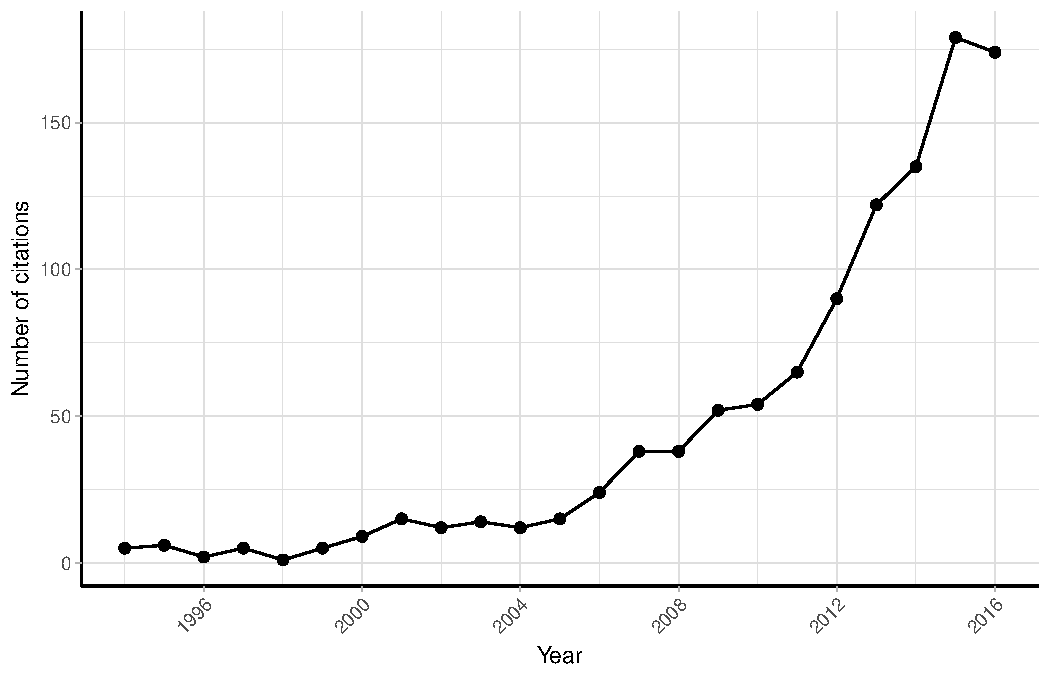
\includegraphics[width=\textwidth]{../figure/cite_grl-1} 

}

\caption[ ]{ }\label{fig:cite_grl}
\end{figure}


\end{knitrout}


% !TeX root = ../kappa.Rnw  


% ---------------------------------------------------------
% Project: PhD KAPPA
% File: aims.tex
% Author: Alessio Crippa
% based on the template written by Andrea Discacciati
%
% Purpose: Aims
% ---------------------------------------------------------

\chapter{Aims of the thesis}

The overall aims of this thesis were to develop and implement new methods for dose--response in meta-analysis, in order to deal with the methodological aspects that have not yet been addressed.

\bigskip

More specifically, the aims were:

\begin{itemize}
\item To describe the implementation of the main aspects of a dose--response meta-analysis and the usage of the \texttt{dosresmeta} $\R$ package.

\item To present and discuss relevant measures and graphical tools to assess the goodness-of-fit in dose--response meta-analysis of binary outcome.

\item To develop a new measure of between-study heterogeneity in the broader context of meta-analysis,  and assess its statistical properties as compared to other available measures. 

\item To explore possible advantages of a point-wise approach, especially, in case of dose--response meta-analysis where the exposure range varies substantially across the studies.

\item To formalize and present an alternative one-stage random-effects model for dose-response meta-analysis of aggregated data, formulating the meta-analytic model in terms of a general linear mixed-effect model. 

\end{itemize}

% !TeX root = ../kappa.Rnw  


% ---------------------------------------------------------
% Project: PhD KAPPA
% File: materials.tex
% Author: Alessio Crippa
% based on the template written by Andrea Discacciati
%
% Purpose: Materials
% ---------------------------------------------------------

\chapter{Materials and methods}

Write materials and methods with subsections as in the background section

% !TeX root = ../kappa.Rnw  

% ---------------------------------------------------------
% Project: PhD KAPPA
% File: results.tex
% Author: Alessio Crippa
% based on the template written by Andrea Discacciati
%
% Purpose: Results
% ---------------------------------------------------------

\chapter{Results}

Write the results with subsections as in the background section


% Paper I
%\input{results.1}

% !TeX root = ../kappa.Rnw  

% ---------------------------------------------------------
% Project: PhD KAPPA
% File: discussion.tex
% Author: Alessio Crippa
% based on the template written by Andrea Discacciati
%
% Purpose: Discussion
% ---------------------------------------------------------

\chapter{Discussion}

Write the discussion with subsections as in the background section

% !TeX root = ../kappa.Rnw  

% ---------------------------------------------------------
% Project: PhD KAPPA
% File: conclusions.tex
% Author: Alessio Crippa
% based on the template written by Andrea Discacciati
%
% Purpose: Conclusions
% ---------------------------------------------------------

\chapter{Conclusions}

The methods presented in this thesis enrich the set of tools available to apply dose--response meta-analyses and to address specific questions including how to evaluate the goodness-of-fit and how to measure the impact of the between-studies heterogeneity. Furthermore, this thesis presents alternative models for pooling results in case of heterogeneous exposure range and for estimating complex models without excluding relevant studies. The proposed methods have been illustrated using real data from published meta-analyses and implemented in the \texttt{dosresmeta} and \texttt{hetmeta} $\R$ packages available on CRAN. 

More specifically we conclude the following:

\begin{itemize}

\item The \texttt{dosresmeta} $\R$ package can help practitioners to conduct dose--response meta-analyses and to apply the methods presented in this thesis. Dedicated functions help to avoid common pitfalls frequently encountered in published meta-analyses, such as definition of the design matrix and prediction of the pooled results (\citetalias{crippadosresmeta2016}).

\item Goodness-of-fit should be regularly evaluated in applied dose-response meta-analysis. The proposed solutions consist of descriptive measures to summarize the agreement between fitted and observed data (the deviance and the coefficient of determination), and graphical tools to visualize the fit of the model (decorrelated residuals-versus-exposure plot). These tools can be employed to identify systematic dose--response patterns and possible source of heterogeneity, and to support the conclusions in applied meta-analyses (\citetalias{discacciati2015goodness}).

\item The new measure of heterogeneity, $R_b$, quantifies the proportion of the variance of the pooled estimate attributable to the between-study heterogeneity. It does not make any assumption about the distribution of the within-study error variances, nor does it require specification of a typical value for these quantities. Therefore, we recommend the use of the $R_b$ as preferred measure for quantifying the impact of heterogeneity (\citetalias{crippa2016new}). 

\item A point-wise strategy for dose-response meta-analysis does not require the specification of a unique model as in the traditional approaches, and thus allows for more flexibility in modeling the individual curves. In addition, the extent of extrapolation is limited by predicting the study-specific relative risk based on the observe exposure range. The use of the described strategy may improve the robustness of the results, especially in case of heterogeneous exposure range (\citetalias{crippa2018pointwise}).

\item A one-stage approach for dose--response meta-analysis consists of a linear mixed-effects model, which offer useful tools for describing the impact of heterogeneity over the exposure range, for comparing the fit of different models, and for predicting individual dose-response associations. The main advantage as compared to a two-stage analysis is that complex curves can be estimated without excluding relevant studies (\citetalias{crippa2018one}).

\end{itemize}

% !TeX root = ../kappa.Rnw  

% ---------------------------------------------------------
% Project: PhD KAPPA
% File: future.tex
% Author: Alessio Crippa
% based on the template written by Andrea Discacciati
%
% Purpose: Future research
% ---------------------------------------------------------

\chapter{Future research}

Based on the conclusions presented in this thesis, future research includes: 

\begin{itemize}
\item <>

\item <>

\item <>
\end{itemize}

% Appendix
\appendix

% !TeX root = ../kappa.Rnw  

% ---------------------------------------------------------
% Project: PhD KAPPA
% File: appendix.tex
% Author: Alessio Crippa
% based on the template written by Andrea Discacciati
%
% Purpose: Appendix
% ---------------------------------------------------------

\chapter{Supplementary figures}

Figures.

%--tables
\chapter{Supplementary tables}

Tables.

% Back matter
\backmatter
\bibliographystyle{style/jss}
\refstepcounter{chapter}
\addcontentsline{toc}{chapter}{\bibname}
\bibliography{additional/kappa_bib}
\newpage
\pagestyle{nothing}

% ---------------------------------------------------------
% Project: PhD KAPPA
% File: acknowledgements.tex 
% Author: Alessio Crippa
% based on the template written by Andrea Discacciati
%
% Purpose: Acknowledgements
% ---------------------------------------------------------

\chapter{Acknowledgements}

There are many people that I would like to thank for their contributions to this thesis, and for their support and encouragement during these years.

\bigskip

\textbf{Nicola Orsini}, my main supervisor for the second half of my doctoral education.

\bigskip

\noindent This work was supported by \textbf{Karolinska Institutet}'s funding for doctoral students (KID-funding).







\end{document}
